\documentclass[conference]{IEEEtran}
\IEEEoverridecommandlockouts
\renewcommand{\thesection}{\Roman{section}}
\usepackage{booktabs}
\usepackage{fancyhdr}
\usepackage[usenames, dvipsnames]{xcolor}
\usepackage{caption}
\usepackage{graphicx}
\usepackage{array}
\usepackage{hyperref,color,float}
\hypersetup{hidelinks,pdfauthor={},pdfcreator={},pdfproducer={},pdftitle={Anonymous submission}}
\usepackage{cite}
\usepackage{multirow}
\usepackage{amsmath,amssymb,amsfonts}
\usepackage{textcomp}
\usepackage{tikz}
\usetikzlibrary{positioning,arrows.meta}

\fancypagestyle{firstpage}{
  \fancyhf{}
  \fancyhead[L]{\small 2027 IEEE 3rd International Conference on Quantum Photonics, Artificial Intelligence, and Networking (QPAIN)\\ 31 March - 03 April, Chittagong, Bangladesh}
  \fancyfoot[L]{\small 979-8-3195-8067-2/27/\$31.00 \copyright2027 IEEE}
  \renewcommand{\headrulewidth}{0pt}
  \renewcommand{\footrulewidth}{0pt}
}
\pagestyle{plain}

\title{Pooling Evidence Over Time Matters More Than the Detector: Catching Mimicking Eavesdroppers in Simulated Fiber-Wireless Links}

\author{\IEEEauthorblockN{Anonymous Authors}
\IEEEauthorblockA{Anonymous Affiliation\\
Anonymous City, Country}}

\begin{document}
\maketitle
\thispagestyle{firstpage}

\begin{abstract}
Fiber-wireless links can be tapped where the light leaves the fiber, and a careful eavesdropper can restore the tapped signal until it looks almost normal. Since a defender never sees examples of such an attack, the usual recommendation is an autoencoder trained on normal traffic that raises an alarm when it cannot reconstruct its input. The comparisons behind that recommendation rarely hold rival detectors to the same false-alarm rate or tune them with equal care, which leaves an operator unable to say whether the autoencoder or the test setup produced the reported gain. We built a simulated fiber link followed by a radio link, added a tap whose hiding level can be set, and compared an autoencoder with four simpler detectors trained on normal data only. In our tests, how a detector pooled evidence over time mattered more than which detector it was. Scored one short window at a time, the detectors were close and the leader changed with the radio channel. Once a running sum over windows was added and tuned without attack data, four of the five caught almost every attack in three of the four channels; the autoencoder pulled clearly ahead only in the hardest one. Almost all of the evidence came from the variance of the received amplitude. A small change in the channel broke the false-alarm control of every detector, so recalibration in the field looks like the harder problem. All results come from simulation.
\end{abstract}

\begin{IEEEkeywords}
fiber-wireless, physical-layer security, eavesdropping detection, anomaly detection, autoencoder, benchmark
\end{IEEEkeywords}

%=====================================================================
\section{Introduction}
Fiber-wireless (FiWi) access networks carry traffic over optical fiber to a handover point, where it is converted and sent on by radio~\cite{tsompanoglou2023}. Bending the fiber or inserting a coupler is enough to tap it, and recent work detects such taps from optical monitoring data~\cite{li2025fiber,qin2026localization,knapinska2025}. A passive tap removes some power, adds a little noise and leaves a weak echo. An attacker who knows this can amplify the stolen signal back to its old level and suppress the rest, much as learned spoofers imitate legitimate radio signals~\cite{shi2021gan}, and the defender is left looking for a small statistical change it has never observed.

Most proposals for this setting use unsupervised learning, often an autoencoder trained on normal data that flags inputs it reconstructs badly. Autoencoders have been reported to work for fiber monitoring~\cite{abdelli2022}, radio authentication~\cite{senigagliesi2025} and spoofing detection~\cite{chen2025mris}, but each of these studies evaluates one method under one calibration. Whether the autoencoder still wins when simpler detectors are held to the same false-alarm rate and tuned just as carefully is seldom checked. For an operator the difference is practical: every false alarm sends a crew to inspect a fiber, and a detector that exceeds its promised false-alarm rate will be switched off however well it detects. If the published advantage comes from an untuned baseline or a looser threshold, the operator pays for a heavier model and gains nothing.

We ran that check on a simulated FiWi link in which a single parameter sets how much of its footprint the attacker hides. Four questions guided the work:
\begin{itemize}
\item \textbf{RQ1.} How fast does detection fall as the attacker hides more?
\item \textbf{RQ2.} Does an autoencoder beat simpler detectors at the same false-alarm rate?
\item \textbf{RQ3.} How much do pooling evidence over time and tuning change the answer?
\item \textbf{RQ4.} Which measured features carry the detection?
\end{itemize}
In brief, detection collapses once the attacker suppresses its excess noise (RQ1). Window by window the autoencoder is sometimes ahead and sometimes behind (RQ2). A tuned running sum lifts most detectors to near-complete detection, leaving the autoencoder ahead in one hard channel (RQ3), and a single amplitude feature does nearly all the work (RQ4). The experiments use six hand-crafted features on simulated data, and we make no claim about real networks.

%=====================================================================
\section{System, Attacker and Detectors}

\begin{figure*}[t]
\centering
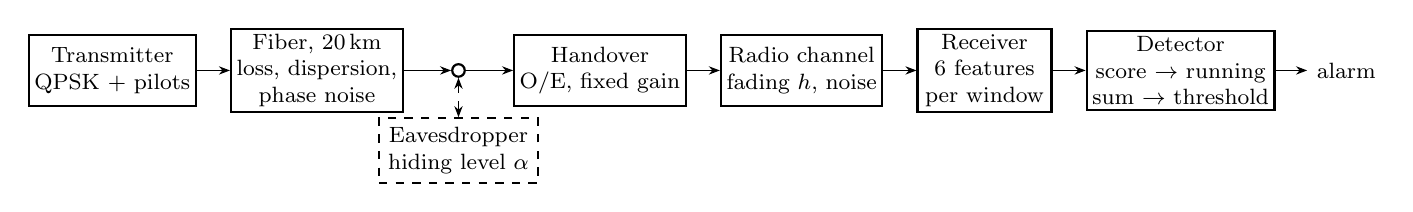
\begin{tikzpicture}[
  font=\footnotesize, >={Stealth[length=4pt]}, node distance=4.2mm,
  blk/.style={draw, thick, minimum height=9mm, minimum width=17mm, align=center, inner sep=2pt}]
\node[blk] (tx) {Transmitter\\QPSK + pilots};
\node[blk, right=of tx] (fib) {Fiber, 20\,km\\loss, dispersion,\\phase noise};
\node[draw, thick, circle, inner sep=1.6pt, right=6mm of fib] (tap) {};
\node[blk, right=6mm of tap] (ho) {Handover\\O/E, fixed gain};
\node[blk, right=of ho] (rad) {Radio channel\\fading $h$, noise};
\node[blk, right=of rad] (rx) {Receiver\\6 features\\per window};
\node[blk, right=of rx] (det) {Detector\\score $\to$ running\\sum $\to$ threshold};
\node[draw, thick, dashed, below=5mm of tap, minimum width=17mm, minimum height=7mm, align=center] (eve) {Eavesdropper\\hiding level $\alpha$};
\draw[->] (tx) -- (fib); \draw[->] (fib) -- (tap); \draw[->] (tap) -- (ho);
\draw[->] (ho) -- (rad); \draw[->] (rad) -- (rx); \draw[->] (rx) -- (det);
\draw[<->, dashed] (tap) -- (eve);
\draw[->] (det.east) -- ++(4mm,0) node[right, align=left] {alarm};
\end{tikzpicture}
\caption{Simulated link. The tap sits at the fiber output, before the handover; the eavesdropper takes 10\% of the power and can reinject a corrected signal. Detectors and thresholds are fitted on normal data only.}
\label{fig:system}
\end{figure*}

\subsection{Link}
Fig.~\ref{fig:system} shows the simulated chain. Symbols are QPSK, grouped in windows of 256 with 32 known pilots per window. The fiber is 20\,km long, with 0.2\,dB/km loss, residual chromatic dispersion (5\% of the 20\,km at 17\,ps/(nm$\cdot$km)), laser phase noise with 100\,kHz linewidth, and additive noise at a signal-to-noise ratio (SNR) of 30\,dB. At the handover a fixed gain undoes the nominal fiber loss, so any change in fiber power reaches the radio side unaltered. The radio segment multiplies each window by one fading coefficient, drawn independently per window (no fading, Rician with $K=5$, or Rayleigh~\cite{goldsmith2005wireless}), and adds receiver noise at the chosen SNR.

\subsection{Attacker}
The tap removes 10\% of the power at the fiber output. It also adds excess noise 30\,dB below the tapped signal and a one-symbol echo of relative amplitude 0.03. The hiding level $\alpha\in[0,1]$ removes these effects in a fixed order: between $\alpha=0$ and 0.5 the attacker restores the power, between 0.5 and 0.75 it removes the excess noise, and between 0.75 and 1 it removes the echo. A passive tap is $\alpha=0$; at $\alpha=1$ nothing is left to detect, so every detector must sit at chance there. Unless stated otherwise we use $\alpha=0.5$, where the power is restored but the noise and echo remain.

\subsection{Features}
The receiver computes six features per window: mean received power; error vector magnitude after pilot-based equalization; magnitude of the pilot-based channel estimate; change of the pilot phase since the previous window (the absolute phase drifts with laser noise); variance of the received amplitude $|r[n]|$; and excess kurtosis of $|r[n]|$. All are standardized with training statistics.

\subsection{Detectors}
Every detector is fitted on normal windows only. \emph{Energy} scores the distance of window power from its normal mean. \emph{Power CUSUM} is a two-sided cumulative sum of standardized power with slack $k=0.5$~\cite{basseville1993}. \emph{PCA} scores the residual after projection on the leading principal components (3 by default). \emph{LOF} uses 20 neighbors~\cite{breunig2000lof}. \emph{OC-SVM} uses an RBF kernel with $\gamma=1/(d\,\mathrm{Var})$ and picks $\nu\in\{0.01,0.05,0.1\}$ by the rejection rate on normal validation data~\cite{scholkopf2001ocsvm}. \emph{Isolation forest} (iForest) has 200 trees~\cite{liu2008iforest}. The \emph{autoencoder} (AE) is a 6--16--3--16--6 network with tanh units, trained with Adam and early stopping on normal validation loss, and scores a window by its reconstruction error.

To pool evidence over time, any score $s_m$ can feed a running statistic $g_m=\max(0,\,g_{m-1}+z_m-k)$, where $z_m$ is $s_m$ standardized with normal validation data and $k\ge0$ is a slack; $k=0$ gives a plain running sum. We mark this wrapper ``+ sum''. Its state is reset at the start of each stream.

\subsection{Two evaluation protocols}
\emph{Window level (P1).} For each seed, 50 independent link realizations are split 60/20/20 into training, validation and test. A test stream has 200 windows and the attack starts at window 100. The threshold is the 99th percentile of validation scores, i.e.\ 1\% false alarms per window. We report the area under the ROC curve (AUC) of attack windows against pre-attack windows and the per-window detection rate $P_d$. The main sweep covers SNR 0--30\,dB in 5\,dB steps, three fading types, five values of $\alpha$, 13 detector variants and 10 seeds.

\emph{Stream level (P2).} An operator acts on an alarm for a stream, and pooled scores are strongly correlated from window to window, so a per-window false-alarm rate flatters pooled detectors. P2 sets the threshold at the $(1-p)$ quantile of the maximum score over 500 normal calibration streams of 100 windows, which gives a false-alarm probability $p$ per 100-window stream, and checks the realized rate on 500 further normal streams. $P_d$ is the fraction of 100 test streams with at least one alarm within 100 windows of onset. We use $p=0.05$ and four channels where the task is neither trivial nor hopeless: no fading, Rician and Rayleigh at 20\,dB, and Rayleigh at 15\,dB. Each family is tuned on seeds 100--104 and tested on fresh seeds 200--204, over PCA components 2--5, LOF neighbors 10/20/50, OC-SVM $\gamma$ scaled by 0.3/1/3, AE hidden width 16/64, 100 or 300 training streams, and either no wrapper or a slack $k$ between 0 and 0.5. The \emph{label-free} rule picks one setting per family: the one that best detects a synthetic anomaly made from normal data (two random features shifted by 0.4 or 0.75 standard deviations), pooled over all channels. Attack data never enter training, thresholds or this tuning. As references only, we report a supervised detector (gradient-boosted trees trained on labelled attack windows, with running sum) and the same families tuned with attack labels.

%=====================================================================
\section{Results}

\begin{figure}[t]
\centering
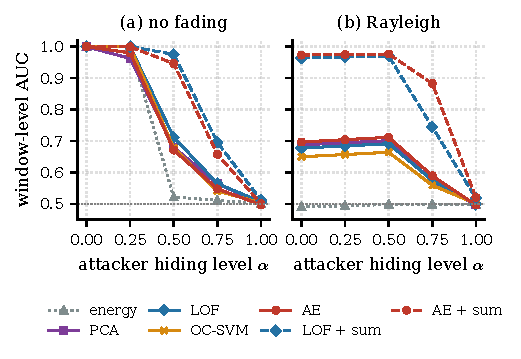
\includegraphics[width=\columnwidth]{figs/fig2_auc_vs_alpha.pdf}
\caption{Window-level AUC against hiding level $\alpha$ at 20\,dB (protocol P1, mean of 10 seeds). Solid: one window at a time. Dashed: with running sum ($k=0.5$). PCA uses 3 components.}
\label{fig:alpha}
\end{figure}

\subsection{Detection versus hiding level (RQ1)}
At 20\,dB without fading (Fig.~\ref{fig:alpha}a), a passive tap ($\alpha\le0.25$) is caught by every detector, the energy detector included. Restoring the power ($\alpha=0.5$) is enough to push energy and power CUSUM to chance (AUC 0.52 and 0.56), whereas the multi-feature detectors hold AUC 0.67--0.71. They drop to 0.54--0.57 once the excess noise is hidden as well ($\alpha=0.75$), and all detectors land at 0.49--0.51 at $\alpha=1$, as the design requires. Rayleigh fading (Fig.~\ref{fig:alpha}b) masks the power drop on its own: the energy detector is at chance even against a passive tap (0.49), while PCA, LOF, OC-SVM and the AE stay at 0.65--0.71 up to $\alpha=0.5$ and iForest at 0.59--0.61. Noise sets a hard limit. At $\alpha=0.5$ and an SNR of 10\,dB or less, every detector, pooled or not, has mean AUC between 0.48 and 0.54, so the rest of the paper works at 15--20\,dB.

\begin{table}[t]
\caption{Window-level results at $\alpha=0.5$, 20\,dB (P1, mean of 10 seeds, threshold at 1\% per-window false alarm).}
\label{tab:window}
\centering
\footnotesize
\setlength{\tabcolsep}{3.2pt}
\begin{tabular}{lcccccc}
\toprule
 & \multicolumn{3}{c}{AUC} & \multicolumn{3}{c}{$P_d$ per window} \\
\cmidrule(lr){2-4}\cmidrule(lr){5-7}
Detector & None & Rician & Rayl. & None & Rician & Rayl. \\
\midrule
Energy        & 0.52 & 0.51 & 0.50 & 0.02 & 0.01 & 0.01 \\
Power CUSUM   & 0.56 & 0.51 & 0.49 & 0.03 & 0.01 & 0.01 \\
\midrule
PCA           & 0.68 & 0.75 & 0.70 & 0.04 & 0.20 & 0.11 \\
LOF           & 0.71 & 0.69 & 0.69 & 0.11 & 0.13 & 0.18 \\
OC-SVM        & 0.68 & 0.67 & 0.66 & 0.10 & 0.14 & 0.16 \\
iForest       & 0.71 & 0.66 & 0.61 & 0.06 & 0.02 & 0.01 \\
AE            & 0.67 & 0.76 & 0.71 & 0.10 & 0.25 & 0.26 \\
\midrule
PCA + sum     & 0.94 & 0.92 & 0.78 & 0.58 & 0.53 & 0.28 \\
LOF + sum     & 0.98 & 0.97 & 0.97 & 0.86 & 0.75 & 0.84 \\
OC-SVM + sum  & 0.97 & 0.97 & 0.98 & 0.83 & 0.83 & 0.88 \\
iForest + sum & 0.97 & 0.89 & 0.78 & 0.82 & 0.51 & 0.22 \\
AE + sum      & 0.95 & 0.97 & 0.98 & 0.75 & 0.85 & 0.89 \\
\bottomrule
\end{tabular}

\smallskip
\parbox{\columnwidth}{\scriptsize Realized per-window false-alarm rate 0.008--0.020 for all rows except PCA, LOF and AE + sum under Rayleigh (0.041--0.043), whose $P_d$ is therefore flattered.}
\end{table}

\subsection{Detectors compared one window at a time (RQ2)}
Table~\ref{tab:window} lists the default detectors at $\alpha=0.5$ and 20\,dB. LOF and iForest lead without fading (AUC 0.71), and the AE comes last of the five (0.67); under fading the order reverses and the AE leads (0.76 Rician, 0.71 Rayleigh). Since all detectors see the same test streams within a seed, we compared them seed by seed. Without fading the AE trails LOF in all 10 seeds (mean difference $-0.041$, 95\% interval $[-0.061,-0.020]$) and cannot be separated from PCA ($-0.009$, $[-0.027,0.010]$). Under Rician fading it beats LOF by 0.070, OC-SVM by 0.093 and PCA by only 0.012 ($[0.009,0.016]$), although that last margin appears in every seed. A consistent 0.012 is a real difference, yet it is far smaller than what a three-component linear projection already achieves, and it reverses when the fading is removed. On this evidence the autoencoder is neither the best nor the worst choice in general.

\subsection{Pooling over time and tuning (RQ3)}
The lower half of Table~\ref{tab:window} shows what a running sum does to the same detectors. LOF, OC-SVM and the AE climb from 0.66--0.76 to 0.95--0.98 in all three channels, while PCA and iForest reach only 0.78 under Rayleigh. After pooling, the AE differs from LOF and OC-SVM by at most 0.03, and none of these paired intervals excludes zero. The autoencoder's small lead under fading did not survive pooling. Stacking the last four windows as input, a cheaper form of memory, helped much less: in a separate run (5 seeds; $\alpha$ 0.25--0.75, three fading types and SNR 10/20/30\,dB pooled) it added 0.03 to mean AUC for the AE and PCA, 0.04 for LOF and 0.05 for OC-SVM, and stacking plus running sum reached 0.78--0.83 for all four. Those means are lower than the 20\,dB values in the table because they include channels where nothing can be detected.

\begin{table}[t]
\caption{Stream-level detection rate $P_d$ at $p=0.05$ false alarms per 100-window stream (P2, $\alpha=0.5$, 5 fresh test seeds). Def.: default settings. +sum: default with running sum, $k=0.5$. LF: tuned without attack data.}
\label{tab:stream}
\centering
\footnotesize
\setlength{\tabcolsep}{3.6pt}
\begin{tabular}{llcccc}
\toprule
 & & None & Rician & Rayl. & Rayl. \\
Family & Setting & 20\,dB & 20\,dB & 20\,dB & 15\,dB \\
\midrule
\multirow{3}{*}{AE}      & Def.  & 0.39 & 0.86 & 1.00 & 0.75 \\
                         & +sum  & 0.80 & 1.00 & 0.87 & 0.85 \\
                         & LF    & 1.00 & 1.00 & 1.00 & \textbf{0.99} \\
\midrule
\multirow{3}{*}{LOF}     & Def.  & 0.82 & 0.56 & 0.58 & 0.12 \\
                         & +sum  & 1.00 & 0.98 & 0.99 & 0.21 \\
                         & LF    & 1.00 & 1.00 & 1.00 & 0.84 \\
\midrule
\multirow{3}{*}{OC-SVM}  & Def.  & 0.74 & 0.48 & 0.91 & 0.15 \\
                         & +sum  & 0.99 & 1.00 & 1.00 & 0.35 \\
                         & LF    & 1.00 & 1.00 & 1.00 & 0.68 \\
\midrule
\multirow{3}{*}{iForest} & Def.  & 0.42 & 0.06 & 0.05 & 0.05 \\
                         & +sum  & 1.00 & 0.91 & 0.57 & 0.16 \\
                         & LF    & 1.00 & 1.00 & 0.97 & 0.47 \\
\midrule
\multirow{3}{*}{PCA}     & Def.  & 0.05 & 0.09 & 0.08 & 0.07 \\
                         & +sum  & 0.84 & 0.59 & 0.19 & 0.08 \\
                         & LF    & 0.49 & 0.10 & 0.09 & 0.15 \\
\midrule
\multicolumn{2}{l}{Energy / power CUSUM} & 0.11/0.12 & 0.04/0.06 & 0.06/0.06 & 0.06/0.06 \\
\multicolumn{2}{l}{Supervised reference} & 1.00 & 1.00 & 1.00 & 1.00 \\
\bottomrule
\end{tabular}

\smallskip
\parbox{\columnwidth}{\scriptsize Realized stream false-alarm rate 0.04--0.07 for every row (mean over seeds). The supervised reference uses attack labels and is not a candidate detector.}
\end{table}

Per-window rates are generous to pooled detectors, so Table~\ref{tab:stream} repeats the comparison at a fixed false-alarm budget per stream, with settings chosen on one set of seeds and tested on another. Under default settings and without a wrapper the leader again changes from cell to cell, LOF without fading and the AE under fading, and some detectors barely work: iForest detects 0.05--0.06 of attacked streams under fading and PCA 0.05--0.09 everywhere. The same iForest, given a running sum, catches every attacked stream without fading, and after label-free tuning it reaches 0.97--1.00 in all three 20\,dB channels.

The label-free rule chose a slack of $k=0$, a plain running sum, for every family. We did not anticipate this, since the slack is normally what keeps a CUSUM from drifting on normal data, but with the threshold set on the stream maximum a persistent attack rewards the plain sum. With it, the AE, LOF, OC-SVM and iForest all detect 0.97--1.00 of attacked streams in the 20\,dB channels, matching the supervised reference, and tuning with attack labels instead gives the same numbers to within 0.01. Settings drawn at random from the same grid do worse at Rayleigh 15\,dB for every family except PCA, most visibly for LOF (0.48 against 0.84), so the tuning step is doing real work.

Rayleigh fading at 15\,dB is the one cell where the families separate. There the tuned AE detects 0.99 of attacked streams, LOF 0.84, OC-SVM 0.68, iForest 0.47 and PCA 0.15, and the AE is ahead of LOF in each of the five test seeds (AE 0.97--1.00; LOF 0.81--0.88). Tightening the budget to $p=0.01$ keeps the AE in front (0.92 against at most 0.47) with more seed-to-seed spread. If the autoencoder has a case in this study, it is this cell.

PCA does not fit the pattern. The synthetic anomaly steers it to a setting that stays at 0.09--0.49 in all four cells, while labelled tuning reaches 1.00 in two of them (no fading and Rayleigh 20\,dB). A synthetic anomaly that looks nothing like the real footprint can mislead selection, and an earlier window-level version of the label-free rule (one synthetic anomaly, no running sum) helped in some channels and hurt in others.

We also changed the attacker. A weaker one ($\alpha=0.3$) gave the same ordering, with the AE first or tied first in every cell (at Rayleigh 15\,dB, AE 0.98 and LOF 0.79). An attacker active for only 5 of every 20 windows lowered detection across the board and reshuffled the order: LOF led without fading (0.87 against 0.80 for the AE), the AE kept the lead at Rayleigh 15\,dB (0.60 against 0.32 for LOF), and there the supervised reference stayed well ahead (0.82). A ranking tuned against one attacker does not automatically carry over to another.

\begin{figure}[t]
\centering
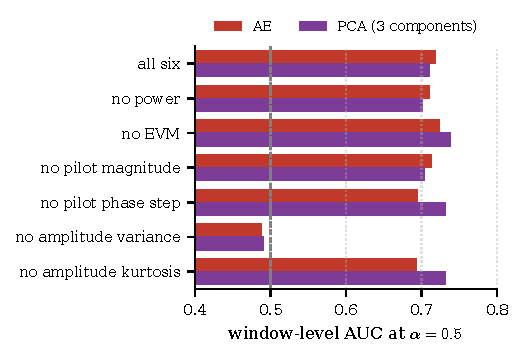
\includegraphics[width=\columnwidth]{figs/fig3_ablation.pdf}
\caption{Leave-one-feature-out at $\alpha=0.5$ (P1, mean of 5 seeds over three fading types and SNR 10/20/30\,dB; default AE, PCA with 3 components). Dashed line: chance (AUC 0.5).}
\label{fig:ablation}
\end{figure}

\subsection{Which features matter (RQ4)}
Removing features one at a time (Fig.~\ref{fig:ablation}) moves mean AUC by at most 0.03 for the AE and PCA, with one exception. Without amplitude variance the AE falls from 0.72 to 0.49 and PCA from 0.71 to 0.49, which is chance, and the same collapse appears in each fading type separately (0.47--0.53). The physics is simple: once the power is restored, what remains of the tap is excess noise and echo, and both widen the distribution of $|r[n]|$. This dependence is specific to the attacker model. In a separate test with an attacker that adds phase jitter instead of noise, dropping amplitude variance did not hurt, and error vector magnitude became the most useful feature.

%=====================================================================
\section{Discussion}

For a defender working with summary features like these, our results suggest an order of work: add a running sum, tune it on normal data, and only then compare models. In our runs that order would have found the autoencoder's one real advantage, at Rayleigh 15\,dB, while avoiding a model change that brought nothing in the easier channels. Raw signal samples might give a learned model more to work with; we did not test that.

The more uncomfortable finding concerns calibration. All thresholds above were set and tested on the same channel. When we moved the channel after calibration, by $\pm3$\,dB in SNR or by a change of fading type (same four channels, 5 seeds, $p=0.05$), the realized false-alarm rate of every pooled detector rose from 0.05 to between 0.33 and 1.00. The supervised reference failed as well, with false alarm 1.00 at $-3$\,dB and $P_d$ 0.00 at $+3$\,dB. Resetting only the threshold on 100 clean streams from the new channel brought false alarms back to 0.05--0.06 but not detection: at $+3$\,dB $P_d$ fell to 0.02--0.05 for all families. A cleaner channel hid the attack: attacked windows scored lower than normal ones, most likely because, at the higher SNR, the tap's excess noise pulled the shifted features back toward the training data. Refitting on 100 shifted streams recovered detection at $+3$\,dB (0.95--1.00), yet at $-3$\,dB it did worse than a threshold reset for every family except iForest. A detector in the field will need clean data from its current channel, and no single repair worked in both directions.

The study has clear limits. All data are simulated, since no FiWi measurements were available to us, and the attacker leaves one family of footprints scaled by one parameter. The six features are hand-crafted and fixed. The window-level sweep (Table~\ref{tab:window}, Fig.~\ref{fig:alpha}) uses 10 seeds, while the ablation, stacking and stream-level runs (Table~\ref{tab:stream}, Fig.~\ref{fig:ablation}) use 5. Detectors within a run share test streams, which makes the comparisons paired. Three of the four stream-level channels are close to saturation, so the evidence that models differ comes mainly from one channel. Finally, the intervals in RQ2 treat seeds as independent and ignore the variance of threshold estimation.

%=====================================================================
\section{Conclusion}
The question behind this study was practical: when no attack data exist, should a FiWi operator reach for an autoencoder to catch a channel-mimicking eavesdropper? Our simulations say that the first decision is how to accumulate evidence across windows and how to tune that step, and that the model can be chosen afterwards; the autoencoder justified itself only in the hardest channel we tried. Two further results matter for anyone building on this work. Detection here hinged on a single amplitude statistic, so a different attacker could leave these detectors blind, and thresholds calibrated on one channel stopped meaning anything after a 3\,dB change. We would encourage future studies to report detectors with and without temporal pooling, at a stated stream-level false-alarm rate, with tuned baselines and seed counts, and to treat recalibration in the field as a research problem of its own. Code and result files will be released after review.

\bibliographystyle{IEEEtran}
\bibliography{refs}

\end{document}
